\documentclass[a4paper, 11pt, final, garamond]{book}
\usepackage{cours-preambule}
\usepackage{pdfpages}

\raggedbottom

\makeatletter
\renewcommand{\@chapapp}{Travaux pratiques -- TP}
\makeatother

\let\SavedIndent\indent
\protected\def\indent{%
  \begingroup
    \parindent=\the\parindent
    \SavedIndent
  \endgroup
}
\setlength{\parindent}{0pt}

\begin{document}
\setcounter{chapter}{30}

\chapter{Mesures de champs magnétiques -- \textsc{Helmoltz} et \textsc{Cotton}}
\begin{center}
  \Large
  \textbf{Objectifs}
\end{center}
\begin{itemize}[label=$\diamond$, leftmargin=10pt]
  \item Mesurer différents ordres de grandeurs de champs magnétiques par
    différentes méthodes.
\end{itemize}

\section{Bobines de \textsc{Helmoltz}}
\label{sec:helm}
\noindent
\begin{minipage}[t]{.45\linewidth}
  Nous allons étudier le champ magnétique créé par deux bobines identiques
  espacées d'une distance $d$ égale à leur rayon.
  \subsection{Réaliser}
  \label{ssec:helmreal}
  \begin{enumerate}
    \item Espacer les deux bobines de $d = R = \SI{6.5}{cm}$
    \item Les brancher \textbf{en série} pour obtenir des champs $\vv{B_1}$ et
      $\vv{B_2}$ de même sens.
    \sqitem[1] Expliquer la démarche expérimentale en quelques lignes.
    \item Fixer $I = \SI{2}{A}$.
    \item Placer la sonde au centre de la bobine de gauche ($x=0$), puis explorer
      le champ pour différentes valeurs de $x$ et compléter le tableau suivant.
  \end{enumerate}
\end{minipage}
\hfill
\begin{minipage}[t]{.45\linewidth}
  ~
  \begin{center}
    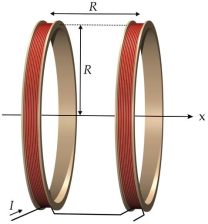
\includegraphics[scale=1]{helm}
    \label{fig:helm}
  \end{center}
\end{minipage}

\begin{table}[h]
  \caption{Tableau à compléter.}
  \label{tab:tofill}
  \centering
  \begin{tabularx}{\linewidth}{|l|Y*{13}{|Y}|}
    \hline
    $x$ (\si{cm}) &
    0 & 1 & 2 & 3 & 4 & 5 & 6 & 7 & 8 & 9 & 10 & 11 & 12 & 13
    \\\hline
    $B$ (\si{mT}) &
    & & & & & & & & & & & & &
    \\
    \hline
  \end{tabularx}
\end{table}

\subsection{Valider et conclure}
\label{ssec:helmval}
% TODO: transport sur Python
\begin{enumerate}[label=\sqenumi, start=2]
  \item Tracer $B = f(x)$ sur Régressi ou LatisPro, imprimer la courbe.
  \item Que dire du champ $\vv{B}$ entre les bobines~?
  \item Faire varier $d$ pour avoir $d \neq R$. Le champ est-il encore uniforme
    entre les bobines~?
  \item Si les bobines étaient parcourues pas des courants de sens contraires,
    que dire de $\vv{B}$ entre les bobines~? Un raisonnement sur les symétries
    est attendu.
\end{enumerate}

\section{La balance de \textsc{Cotton}}
\label{sec:cotton}
\subsection{S'approprier}
\label{ssec:cottonapp}

La balance de \textsc{Cotton} est un dispositif ancien, développé au tout début
du \textsc{xx}\ieme~siècle par Aimé \textsc{Cotton} pour mesurer avec précision
des champs magnétiques. Elle est constituée de deux bras rigidement liés l'un à
l'autre en $\Or$. La partie de gauche comprend sur sa périphérie un conducteur
métallique qui est parcouru par un courant et dont une partie est placée dans le
champ magnétique uniforme et permanent à mesurer, représenté par la zone grisée.
Dans cette partie, les conducteurs aller et retour sont des arcs de cercle de
centre $\Or$, reliés par une portion horizontale de longueur $L$. Le partie
droite comporte un plateau sur lequel est déposée une masse $m$ afin
d’équilibrer la balance.

\noindent
\begin{minipage}[t]{.45\linewidth}
  ~
  \begin{center}
    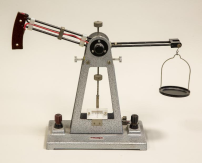
\includegraphics[scale=1]{cottonphot}
    \label{fig:cottonphot}
  \end{center}
\end{minipage}
\hfill
\begin{minipage}[t]{.45\linewidth}
  ~
  \begin{center}
    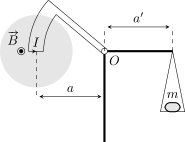
\includegraphics[scale=1]{cottonlang}
    \label{fig:cottonlang}
  \end{center}
\end{minipage}
\bigbreak
La balance peut tourner sans frottements dans le plan de la figure autour du
point $\Or$. À vide, c'est-à-dire sans champ magnétique ni masse $m$, la
position du plateau est ajustée afin que la balance soit à l'équilibre avec le
bras de droite parfaitement horizontal.

\begin{enumerate}
  \sqitem[6] En utilisant des coordonnées cylindriques de centre $\Or$ et d'axe $\Or
    z$ tel que $\vv{B} = B\ez$, montrer que le moment en $\Or$ des forces de
    \textsc{Laplace} s'exerçant sur les parties en arc de cercle est nul.
  \sqitem[7] À l'équilibre, en présence de courant et de champ magnétique,
  établir l'expression du moment en $\Or$ des forces de \textsc{Laplace}. On
  utilisera le bras de levier.
  \sqitem[8] En déduire la relation entre la masse $m$ à poser sur le plateau
  pour retrouver la configuration d'équilibre et le champ magnétique $B$, à
  exprimer en fonction de $a$, $a'$, $L$, $m$ et $g$ l'intensité de la
  pesanteur.
\end{enumerate}

\subsection{Réaliser et valider}
\label{ssec:cottonreal}
\begin{enumerate}
  \item Alimenter le circuit en faisant attention au sens du courant.
  \item Placer sur le plateau une masse de \SI{0.1}{g}.
  \item Régler le courant pour que l'aiguille de la balance soit au centre.
  \sqitem[9] Sachant que dans notre cas, $a' = a$, en déduire la valeur du
  champ magnétique créé par l'aimant.
  \sqitem[10] Vérifier la valeur calculée en mesurant directement le champ
  magnétique grâce à un teslamètre.
\end{enumerate}

\end{document}
